%\section{Списки}
\begin{frame}[plain, noframenumbering]
    \begin{center}
        \Huge
         Проектирование детектора солнечных космических лучей
    \end{center}
\end{frame}
%
%\subsection{Нумерованные}
%
\begin{frame}
    \frametitle{Проектирование детектора солнечных космических лучей}
                \begin{columns}
    	\begin{column}{0.6\textwidth}
    		\textbf{Цели:}
    		\begin{itemize}
    			\item Исследование солнечных космических лучей и
    			солнечных вспышек;
    			\item Обеспечение радиационной безопасности для космонавтов
    			и электроники;
    		\end{itemize}
    		\textbf{Задачи:}
    		\begin{itemize}
    			\item Разработка и оптимизация схемы детектора;
    			\item Методики анализа в разных режимах работы;
    		\end{itemize}
    	\end{column}
    	\begin{column}{0.4\textwidth}
    		\textbf{Требования:}
    	\begin{itemize}
    			\item Протоны от 10 МэВ до 100 МэВ;
    			\item Электроны от 1 МэВ до 10 МэВ;
    			\item Загрузки от $10^6$ Гц;
    			\item Канал связи 1-10 МБ/сутки;
    			\item Размеры  8 см х 6 см х 6 см;
    			\item Масса до 700 грамм.
    	\end{itemize}
    	\end{column}
    \end{columns} 
\end{frame}

\begin{frame}
\frametitle{Проектирование детектора солнечных космических лучей}
\begin{columns}
	\begin{column}{0.4\textwidth}
        \includegraphics[width=1\textwidth]{satellite/poster_1/detector.png}
		\textbf{Сцинтилляционный cегментированный детектор c SiPM:}
	\end{column}
	\begin{column}{0.6\textwidth}
		\begin{itemize}
			\item Определение энергии и типа частиц по распределению ионизационных потерь по глубине детектора.
		\end{itemize}
    Режимы работы:
    \begin{itemize}
        \item Одночастичный (счетный) режим работы для загрузок менее $10^4 - 10^5$ Гц
        \item Интегральный режим (при загрузках $>10^6$ Гц и узких каналах связи)
    \end{itemize}
%		
	\end{column}
\end{columns} 
\end{frame}


\begin{frame}
\frametitle{Проектирование детектора солнечных космических лучей}
\begin{columns}
    \begin{column}{0.5\textwidth}
        \textbf{Одночастичный режим:}
        \includegraphics[width=1\textwidth]{satellite/poster_1/resolution.pdf}
        \begin{itemize}
             \tiny{\item М. Е. Зелёный et al., ПРОЕКТИРОВАНИЕ ДЕТЕКТОРА ПРОТОНОВ И ЭЛЕКТРОНОВ ДЛЯ МОНИТОРИНГА СОЛНЕЧНЫХ КОСМИЧЕСКИХ ЛУЧЕЙ, КСФ ФИАН номер 1, 2019 г.}
            \item \tiny{Prototype of a segmented scintillator detector for particle flux measurements on spacecraft, Препринт, https://arxiv.org/abs/2005.02620}
        \end{itemize}
        
        
   
    \end{column}
    \begin{column}{0.5\textwidth}
        \textbf{Интегральный режим:}
        \includegraphics[width=0.9\textwidth]{satellite/poster_1/Pow.pdf}
        \includegraphics[width=0.9\textwidth]{satellite/poster_1/Gauss.pdf}
        %
             \tiny{   \begin{itemize}
            \item 	M. Zelenyi, M. Poliakova, A. Nozik and A. Khudyakov, Application of Turchin's method of statistical regularization, EPJ Web Conf. Volume 177, 2018
        \end{itemize}}	
    \end{column}
\end{columns} 
\end{frame}


\begin{frame}[plain, noframenumbering]
\begin{center}
	\Huge
	Моделирования сканера транспортных контейнеров
\end{center}
\end{frame}

\begin{frame}
\frametitle{Моделирования сканера транспортных контейнеров}
\begin{columns}
	\begin{column}{0.7\textwidth}
		\begin{block}{Поглощение гамма-квантов}
		$$
		T(E_0, t, Z) = \frac{\int \limits_0^{E_0} S(E_0, E) \exp(-\mu(E,Z)\times t)~dE)}{\int \limits_0^{E_0} S(E_0, E)~dE}
		$$
	\end{block}
		%            \hline
%		\includegraphics[width=1\textwidth]{}
    \begin{block}{Метод дуальных энергий}
    	$$
    	F(z) = \frac{|t(E^{(1)}_0,z) - t(E^{(2)}_0,z)|}{t(E^{(1)}_0,z)} \to min
    	$$
\end{block}
	\end{column}
	\vline~
	\begin{column}{0.4\textwidth} 
		$T$ -  transmittance\\
		$S(E_0, E)$ - response function\\
		$\mu(E,Z)$ - attenuation\\
		$t$ -  optical thickness\\
		$E_0$ -  up-limit energy of bremsstrahlung\\
		$E$ - energy of gamma ray\\
		$Z$ - charge of nuclei 
		%            \hline
        
        \includegraphics[width=1\textwidth]{scanner/Attenuation.pdf}
	\end{column}
\end{columns}  
\end{frame}

\begin{frame}
\frametitle{Моделирования сканера транспортных контейнеров}
\begin{block}{Недостатки метода дуальных энергий}%<1>
	\begin{itemize}
		\item Усложнение конструкции облучателя.
		\item Низкая эффективность если материалы состоят из атомов с сильно различающимися зарядовыми числами.
	\end{itemize}
\end{block}
\begin{block}{Наши предложения}%<2>
	Использовать монохроматический электронный пучок, но при этом измерять энергетическое распределение гамма-квантов.
\end{block}
\begin{block}{Задачи}%<2>
	Моделирование энергетического спектра гамма-квантов при облучении контейнера.
\end{block}
\end{frame}

\begin{frame}
\frametitle{Моделирования сканера транспортных контейнеров}
\begin{columns}
    \begin{column}{0.5\textwidth}
        \includegraphics[width=1\textwidth]{scanner/yed_schema_1.pdf}
        \includegraphics[width=1\textwidth]{scanner/diffmat.pdf}
    \end{column}
    \vline~
    \begin{column}{0.5\textwidth} 
        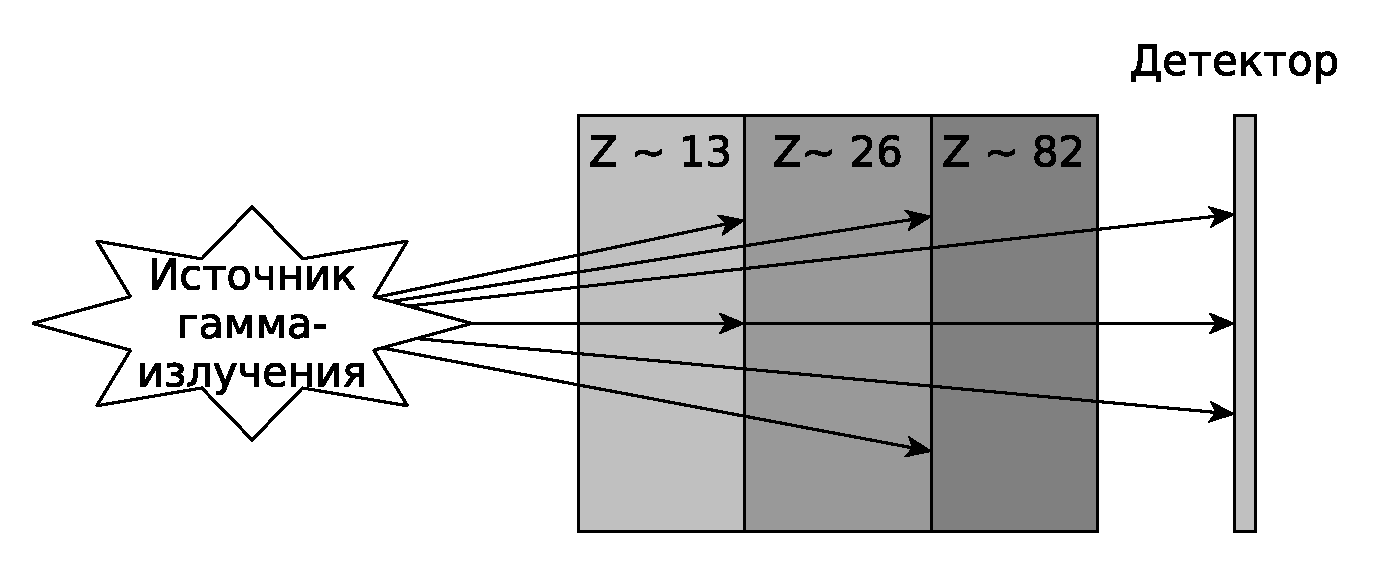
\includegraphics[width=1\textwidth]{scanner/yed_schema_2.pdf}
        \includegraphics[width=1\textwidth]{scanner/reconstruction.pdf}
    \end{column}
\end{columns}  

\tiny {Зелёная А. В., Зелёный М. Е., Туринге А. А., Недорезов В. Г., Анализ химического состава при сканировании транспортных контейнеров гамма-излучением, Физика элементарных частиц и атомного ядра (ЭЧАЯ) выпуск 5, 2019 г.}
\end{frame}



\begin{frame}[plain, noframenumbering]
\begin{center}
    \Huge
   Моделирование лавин релятивистских убегающих электронов в грозовой атмосфере
\end{center}
\end{frame}

\begin{frame}
\frametitle{Моделирование RREA}
\begin{columns}
    \begin{column}{0.5\textwidth}
        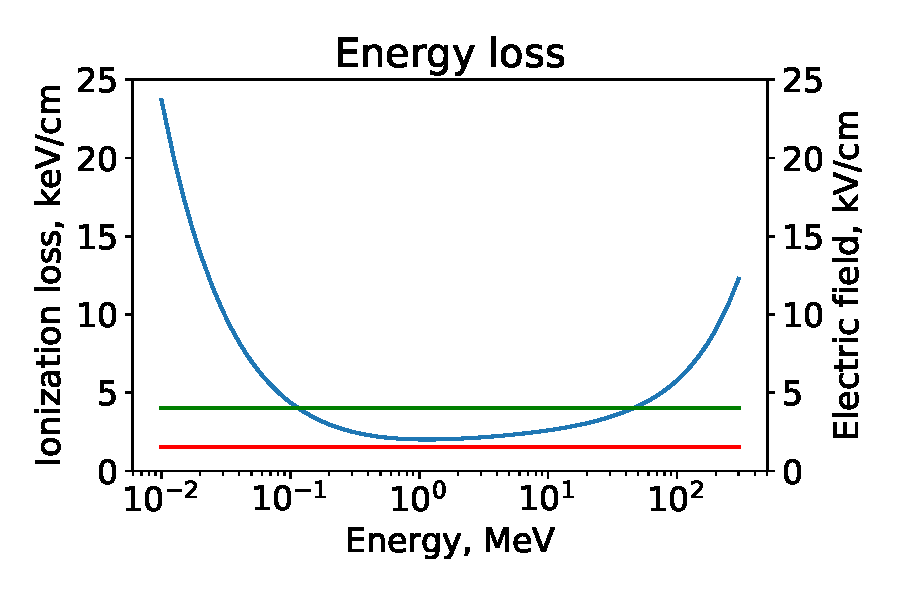
\includegraphics[width=1\textwidth]{thunderstorm/01_Gurevich.pdf}
        \begin{itemize}
            \item \textbf{RB/RREA} - лавины убегающих электронов
        \end{itemize}
    \end{column}
    \vline~
    \begin{column}{0.5\textwidth} 
        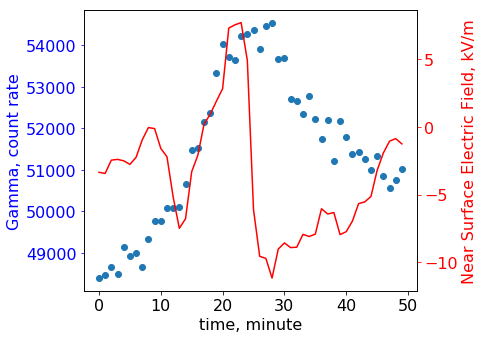
\includegraphics[width=1\textwidth]{thunderstorm/ayss_2019_pres/aragats.png}
        \begin{itemize}
           \item \textbf{TGF} - короткие (~10 мкс) вспышки гамма- и рентгеновского излучения из грозового облака
           \item \textbf{TGE} - длительное (~5 минут) повышение гамма-фона, коррелирующее с изменениями электрического поля
        \end{itemize}

    \end{column}
\end{columns}  
\end{frame}

\begin{frame}
\frametitle{Моделирование RREA}
  \begin{block}{Задачи}
      \begin{itemize}
          \item Моделирование электронной лавины, расчеты числа убегающих электронов.
          \item Изучение влияние гамма-квантов и позитронов на возникновение обратной связи
          \item Создание новых моделей RREA в грозовых облаках.
      \end{itemize}
  \end{block}
{\tiny \begin{itemize}
   \item A.CHILINGARIAN et al., “Structures of the intracloud electric field supporting origin of long-lasting thunderstorm ground enhancements”, PHYS. REV. D 98, 082001 (2018)
   \item M. Zelenyi et al., Estimation of number of runaway electrons per avalanche in earth's atmosphere, Препринт
\end{itemize} }
\end{frame}

\begin{frame}
\frametitle{Моделирование RREA}
\begin{columns}
    \begin{column}{0.5\textwidth}
          \includegraphics[width=0.8\textwidth]{thunderstorm/ayss_2018_art/10_dwyer.pdf}
          
          \tiny{M. Zelenyi, E. Stadnichuk, A. Nozik, Calculation of gain coefficient in Dwyer relativistic discharge feedback model of thunderstorm runway breakdown, EPJ Web Conf. Volume 201, 2019}
    \end{column}
    \vline~
    \begin{column}{0.5\textwidth} 
        Модель Дваера:
          \begin{block}{Нормальные условия}
             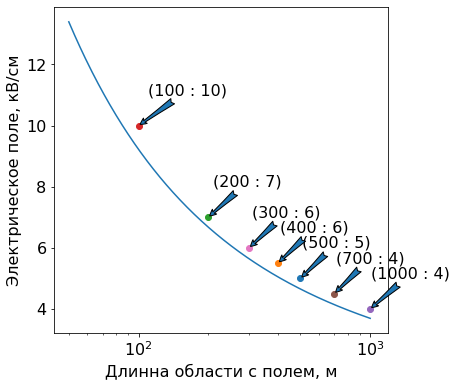
\includegraphics[width=0.8\textwidth]{thunderstorm/dwyer2003.png}
          \end{block}
%        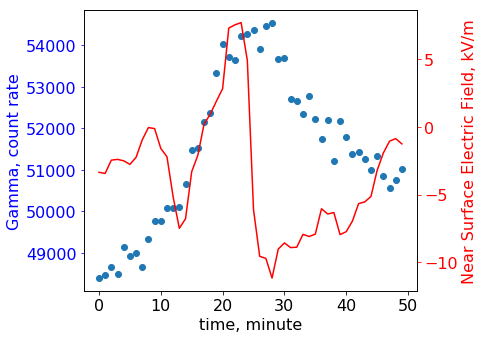
\includegraphics[width=1\textwidth]{thunderstorm/ayss_2019_pres/aragats.png}
          \begin{block}{Высота 5 км}
               \includegraphics[width=0.8\textwidth]{thunderstorm/ayss_2018_art/08_gain.pdf}
          \end{block}

    \end{column}
\end{columns}  
\end{frame}


\begin{frame}
\frametitle{Моделирование RREA}
\begin{columns}
    \begin{column}{0.5\textwidth}
        Затухание:
        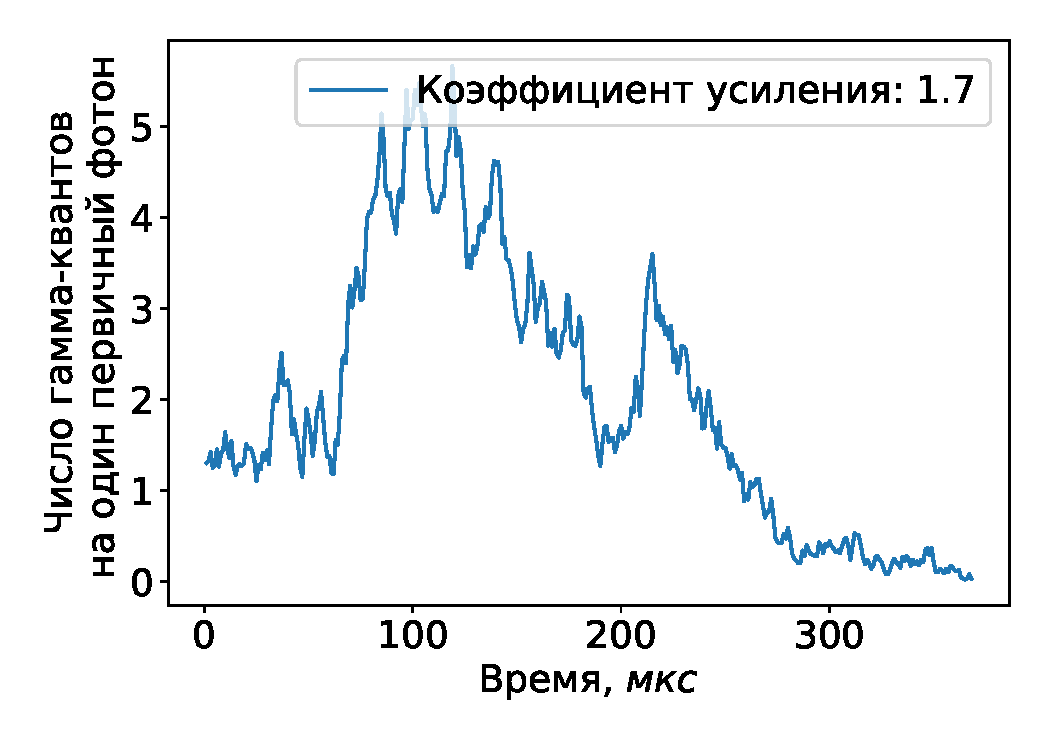
\includegraphics[width=1\textwidth]{thunderstorm/RL_Extinction.pdf}
 {\footnotesize \begin{itemize}
            \item Гамма-кванты с фиксированной длинно свободного пробега.
            \item Рождение гамма-квантов подчинено закону Пуассона.
            \item Направление определяется по полю.
            \item Направление поля случайное.
        \end{itemize}}
    \tiny{M. Zelenyi, E. Stadnichuk, A. Nozik, Reactor like TGE model, AIP Conference Proceedings 2163, 060005 (2019)}
    
%        \includegraphics[width=1\textwidth]{thunderstorm/diffmat.pdf}
    \end{column}
    \vline~
    \begin{column}{0.5\textwidth} 
        TGE:
        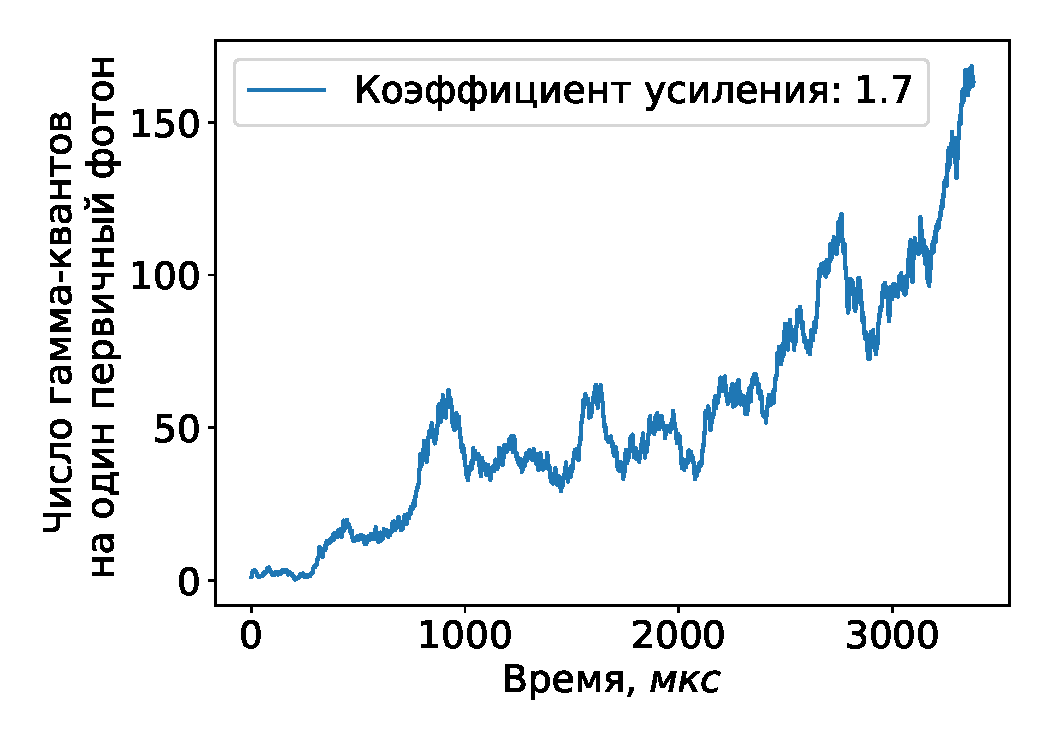
\includegraphics[width=1\textwidth]{thunderstorm/RL_proofTGE.pdf}
        TGF:
        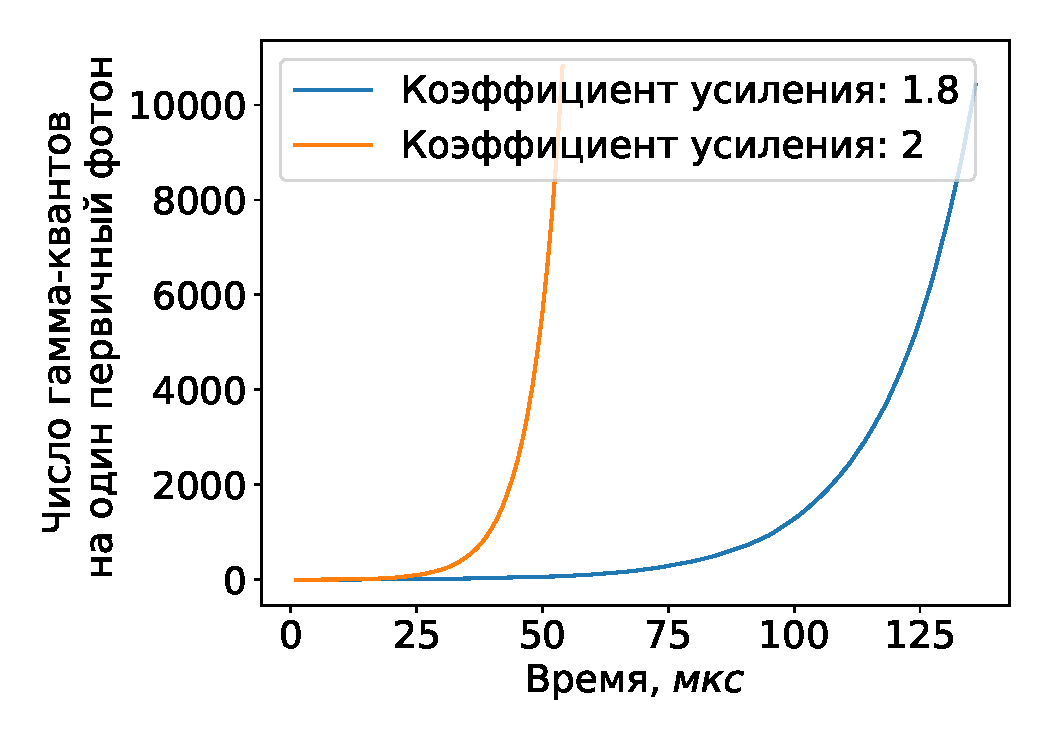
\includegraphics[width=1\textwidth]{thunderstorm/RL_proofTGF.pdf}
    \end{column}
\end{columns}  
\end{frame}



%\note{
%    Этот текст будет виден только если его отображение включено в файле \textbf{Presentation/setup}.
%    Для раздельного вывода презентации и заметок на разные экраны (как в impress или powerpoint) можно использовать программу \textit{pdf-presenter-console}.
%}
%
%\subsection{Не нумерованные}
%
%
%\begin{frame}
%    \frametitle{Перечисления}
%    \begin{itemize}
%        \item Проблема 1
%        \item Проблема 2
%        \item Проблема 3
%    \end{itemize}
%\end{frame}
%\note[itemize]{
%    \item Тезис 1
%    \item Тезис 2
%    \item Тезис 3
%}


